\documentclass{beamer}
%
% Choose how your presentation looks.
%
% For more themes, color themes and font themes, see:
% http://deic.uab.es/~iblanes/beamer_gallery/index_by_theme.html
%
\mode<presentation>
{
  \usetheme{Madrid}      % or try Darmstadt, Madrid, Warsaw, ...
  \usecolortheme{seahorse} % or try albatross, beaver, crane, ...
  \usefonttheme{serif}  % or try serif, structurebold, ...
  \setbeamertemplate{navigation symbols}{}
  \setbeamertemplate{caption}[numbered]
} 

\usepackage[english]{babel}
\usepackage{kotex}
%\usepackage[utf8x]{inputenc}

\title[게임수학 - 벡터기초]{ 게임 수학 강의 노트 02 - 벡터 기초}
\author{강영민}
\institute{동명대학교}
\date{2016년 2학기}

\begin{document}

%%%%%%%%%%%%%%%%%%%%%%%%%%%%%%%%%%%%%%%%%%%%%%%%%%%%%%%%%
\begin{frame}
  \titlepage
\end{frame}

% Uncomment these lines for an automatically generated outline.
%\begin{frame}{Outline}
%  \tableofcontents
%\end{frame}


%%%%%%%%%%%%%%%%%%%%%%%%%%%%%%%%%%%%%%%%%%%%%%%%%%%%%%%%%
\begin{frame}{벡터란 무엇인가?}
\begin{itemize}
\item 벡터의 의미
  \begin{itemize}
  \item 벡터(vector)는 ‘나르다’라는 의미의 라틴어 동사 ‘vehere'에서 유래
  \item ‘무엇인가를 나르는 것’이라는 의미
  \item 벡터라는 것은 무엇인가를 옮겨 놓는 역할을 수행한다.
  \end{itemize}
\end{itemize}

\begin{itemize}
\item 수학과 물리학에서의 개념
  \begin{itemize}
  \item 크기와 방향으로 결정되는 양(量, quantity)
  \item 방향량(方向量)이라고도  함.
  \item 예: 힘(force)은 크기만으로는 그 성질을 온전히 표현할 수 없고, 방향도 같이 고려해야 하므로 벡터로 표현된다.
  \end{itemize}
\end{itemize}

\begin{block}{벡터}
수학자들은 자연 현상의 많은 것들이 수로 표현될 수 있음을 알았는데, 하나의 숫자로 충분히 표현할 수 있지만 하나 이상의 수가 필요한 경우도 있다. 
이러한 양을 벡터(vector)라고 부른다.
\end{block}

\end{frame}

%%%%%%%%%%%%%%%%%%%%%%%%%%%%%%%%%%%%%%%%%%%%%%%%%%%%%%%%%


%%%%%%%%%%%%%%%%%%%%%%%%%%%%%%%%%%%%%%%%%%%%%%%%%%%%%%%%%
\begin{frame}{벡터의 개념}

\begin{itemize}
\item 물리적 현상 등을 표현할 때 - 대상을 양(量, quantity)으로 표현 
\item 이 양은 스칼라(scalar) 혹은 벡터(vector)
	\begin{itemize}
	\item 스칼라 값은 오로지 크기만으로 완전히 그 양을 표현할 수 것으로서 물체의 질량, 소요된 시간, 길이, 열량 등이 해당
	\item 벡터(vector)는 이와 달리 크기와 함께 방향도 같이 존재하는 양으로 힘, 속도, 변위와 같은 양이 바로 여기에 해당
	\end{itemize}
\end{itemize}

\begin{itemize}
\item 속도(速度, velocity)와 속력(速力, speed)
\item 속도는 벡터, 속력은 스칼라
\end{itemize}

\begin{figure}
\begin{tabular}{c}
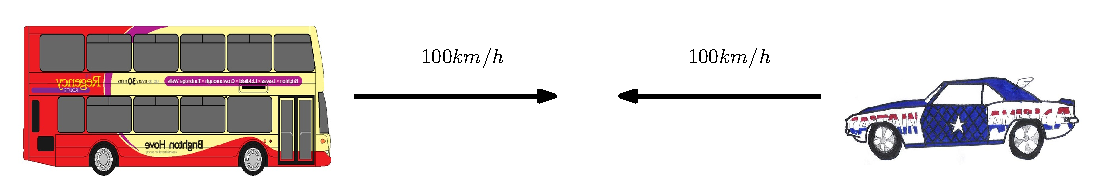
\includegraphics[width=9.25cm]{./Math_vector/movingVehicles.eps} \\
{\tiny 동일한 속력으로 서로 마주 보며 달리는 차량의 속도 }
\end{tabular}
\end{figure}
\end{frame}
%%%%%%%%%%%%%%%%%%%%%%%%%%%%%%%%%%%%%%%%%%%%%%%%%%%%%%%%%

%%%%%%%%%%%%%%%%%%%%%%%%%%%%%%%%%%%%%%%%%%%%%%%%%%%%%%%%%
\begin{frame}{화살표를 이용한 벡터 표현}
\begin{itemize}
\item 벡터를 표현하는 가장 직관적인 방법은 화살표를 이용
\item 화살표: 시점(始點)과 종점(終點)으로 구성 
\item 화살표의 방향은 벡터의 방향을 시각적으로 표현하고, 화살표의 길이는 벡터의 크기를 시각적으로 표현
\end{itemize}

\begin{figure}
\begin{tabular}{c}
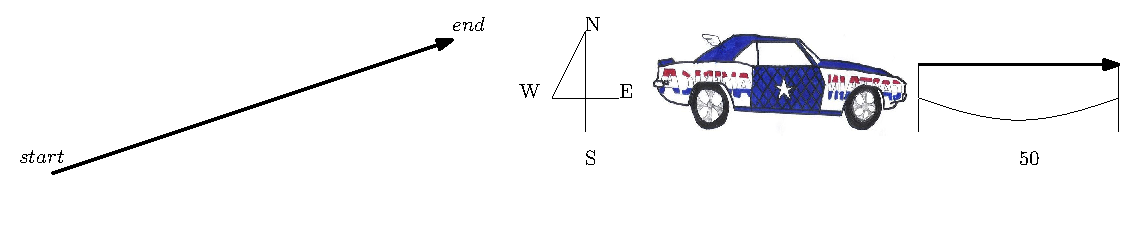
\includegraphics[width=8cm]{Math_vector/vectorExpression.eps}\\
{\tiny 벡터의 시각적 표현과 달리는 자동차 속도 표현의 예}
\end{tabular}
\end{figure}

\begin{figure}
\begin{tabular}{c}
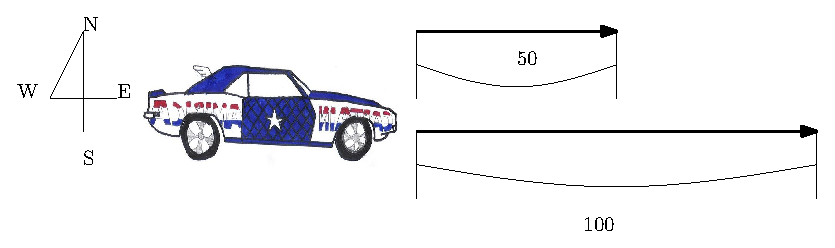
\includegraphics[width=8cm]{Math_vector/increasedSpeed.eps}\\
{\tiny 속력이 두 배로 늘어난 자동차의 속도}
\end{tabular}
\end{figure}

\end{frame}
%%%%%%%%%%%%%%%%%%%%%%%%%%%%%%%%%%%%%%%%%%%%%%%%%%%%%%%%%

%%%%%%%%%%%%%%%%%%%%%%%%%%%%%%%%%%%%%%%%%%%%%%%%%%%%%%%%%
\begin{frame}{동등벡터(equivalent vector)}

\begin{itemize}
\item 벡터의 표기법
\begin{itemize}
\item $\vec{a}$, $\mathbf a$
\end{itemize}
\end{itemize}

\begin{itemize}
\item 동등벡터
\begin{itemize}
\item 크기와 방향이 같으면 모두 동등한 벡터로 간주
\end{itemize}
\end{itemize}

\begin{figure}
\begin{tabular}{c}
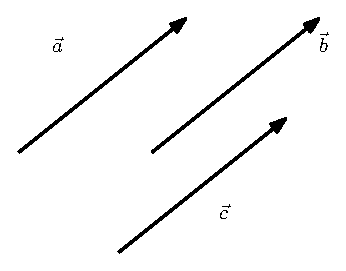
\includegraphics[width=5cm]{Math_vector/equivalentVectors.eps}\\
{\tiny 동등벡터}
\end{tabular}
\end{figure}

\end{frame}
%%%%%%%%%%%%%%%%%%%%%%%%%%%%%%%%%%%%%%%%%%%%%%%%%%%%%%%%%

%%%%%%%%%%%%%%%%%%%%%%%%%%%%%%%%%%%%%%%%%%%%%%%%%%%%%%%%%
\begin{frame}{동등벡터 찾기}

\begin{figure}
\begin{tabular}{c}
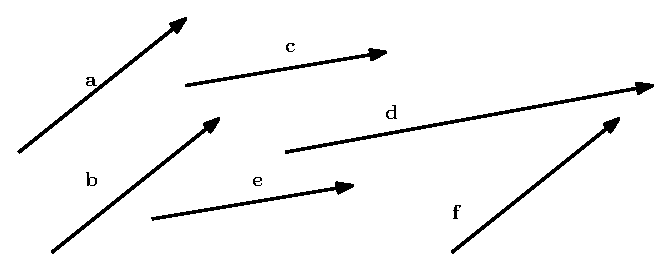
\includegraphics[width=10cm]{./Math_vector/equivalentVectors2.eps}\\
{\tiny 동등벡터 찾기}
\end{tabular}
\end{figure}

\end{frame}
%%%%%%%%%%%%%%%%%%%%%%%%%%%%%%%%%%%%%%%%%%%%%%%%%%%%%%%%%

%%%%%%%%%%%%%%%%%%%%%%%%%%%%%%%%%%%%%%%%%%%%%%%%%%%%%%%%%
\begin{frame}{벡터의 수학적 표현}

\begin{itemize}
\item 벡터: 화살표가 그려지는 공간의 차원(次元,dimension)에 따라 결정되는 개수의 성분
	\begin{itemize}
	\item $n$-튜플(tuple)
	\item $\mathbf v = ( v_1 , v_2 , v_3, \cdots , v_n )$
	\item $n$ 개의 차원을 가진 공간에서 그려지는 화살표 = $n$차원 벡터
	\end{itemize}
\end{itemize}

\end{frame}
%%%%%%%%%%%%%%%%%%%%%%%%%%%%%%%%%%%%%%%%%%%%%%%%%%%%%%%%%


%%%%%%%%%%%%%%%%%%%%%%%%%%%%%%%%%%%%%%%%%%%%%%%%%%%%%%%%%
\begin{frame}{2차원 벡터}

\begin{figure}[h!]
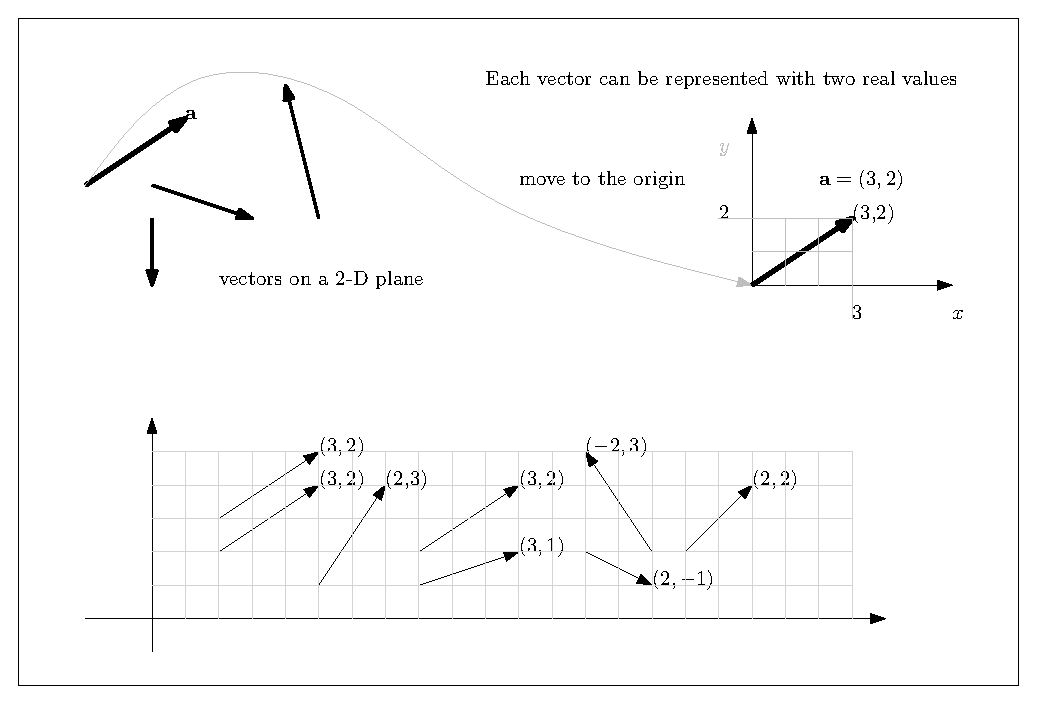
\includegraphics[width=10cm]{Math_vector/2dVectors.eps}
\end{figure}
\end{frame}
%%%%%%%%%%%%%%%%%%%%%%%%%%%%%%%%%%%%%%%%%%%%%%%%%%%%%%%%%


%%%%%%%%%%%%%%%%%%%%%%%%%%%%%%%%%%%%%%%%%%%%%%%%%%%%%%%%%
\begin{frame}{시점을 원점으로 옮기기}
시점이 원점이 아닌 벡터는 시점을 원점으로 끌어 오면 된다.
벡터의 시점은 (3,6)의 좌표에 놓여있고, 끝점은 (16,9)이다. 시작점을 원점으로 옮기는 것은 (-3,-6) 만큼의 이동을 하는 것이다.
따라서 끝점은 (13,3)의 위치로 이동하게 된다. 그러므로 이 벡터는 (13,3)으로 표현된다.

\begin{figure}
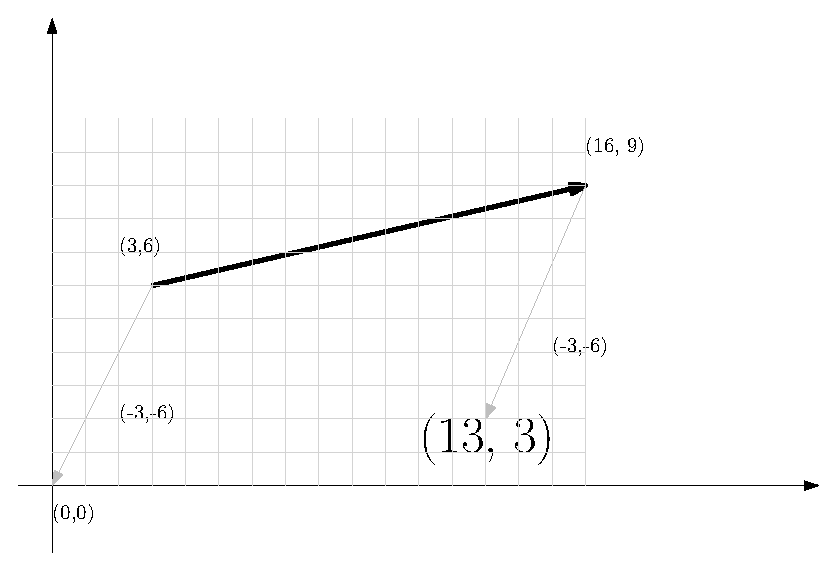
\includegraphics[width=9cm]{Math_vector/vectorMove.eps}
\end{figure}

\end{frame}
%%%%%%%%%%%%%%%%%%%%%%%%%%%%%%%%%%%%%%%%%%%%%%%%%%%%%%%%%

%%%%%%%%%%%%%%%%%%%%%%%%%%%%%%%%%%%%%%%%%%%%%%%%%%%%%%%%%
\begin{frame}{3차원 벡터}
3차원 벡터는 지금까지 살펴본 2차원 벡터에 축(軸, axis)을 하나 더하기만 하면 된다.
\begin{figure}
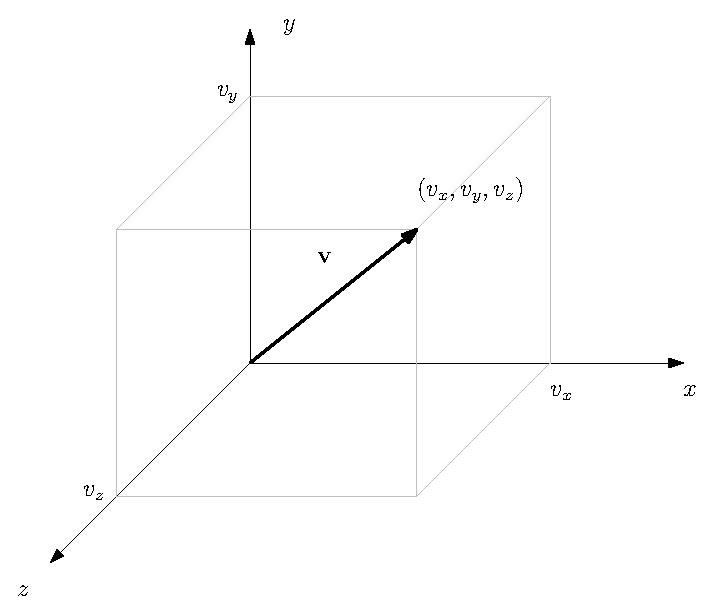
\includegraphics[width=9cm]{Math_vector/3dVector.eps}
\end{figure}
\end{frame}
%%%%%%%%%%%%%%%%%%%%%%%%%%%%%%%%%%%%%%%%%%%%%%%%%%%%%%%%%


%%%%%%%%%%%%%%%%%%%%%%%%%%%%%%%%%%%%%%%%%%%%%%%%%%%%%%%%%
\begin{frame}{벡터의 크기}
\begin{figure}
\begin{tabular}{p{6cm}p{5cm}}
\raisebox{-\totalheight}{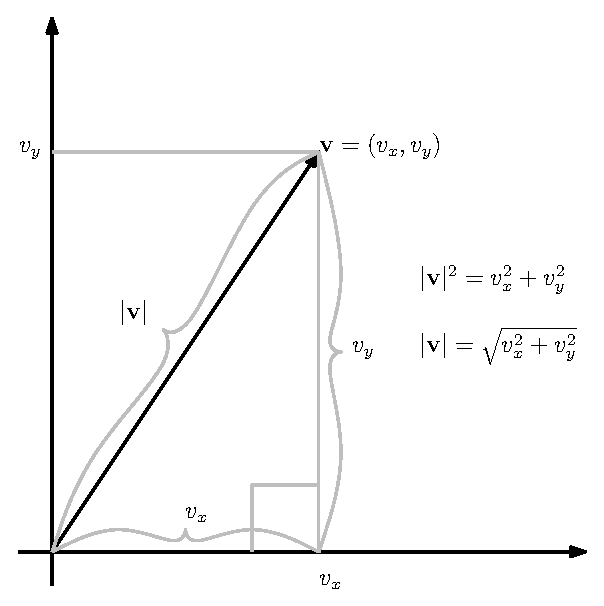
\includegraphics[width=6cm]{Math_vector/Pythagoras2D.eps}}
&
어떤 벡터 $\mathbf v$가 $(v_x , v_y )$로 표현될 때 
이 벡터의 크기는 $v_x$와 $v_y$로 어떻게 구할 수 있을까?
그 값은 '길이'에 대한 상식적 정의에 따라, 스칼라 값이며 양(陽, positive)의 값이 된다.
이렇게 양의 길이(positive length)를 벡터에 할당하는 것을 놈(norm)이라 하며, 
어떤 벡터 $\mathbf v$의 놈은 $|| \mathbf v ||$로 표현한다.
유클리드 기하에 의해 얻어지는 길이는 Euclidean Norm이라고 한다.
이는 피타고라스의 정리를 이용하여 쉽게 구할 수 있다.
\end{tabular}
\end{figure}
\end{frame}
%%%%%%%%%%%%%%%%%%%%%%%%%%%%%%%%%%%%%%%%%%%%%%%%%%%%%%%%%

%%%%%%%%%%%%%%%%%%%%%%%%%%%%%%%%%%%%%%%%%%%%%%%%%%%%%%%%%
\begin{frame}{3차원 벡터의 크기}
\begin{eqnarray}
\mathbf v = (v_x , v_y, v_z) \nonumber \\
|| \mathbf v || = \sqrt{v_x^2 + v_y^2 + v_z^2} \nonumber
\end{eqnarray}

\begin{figure}
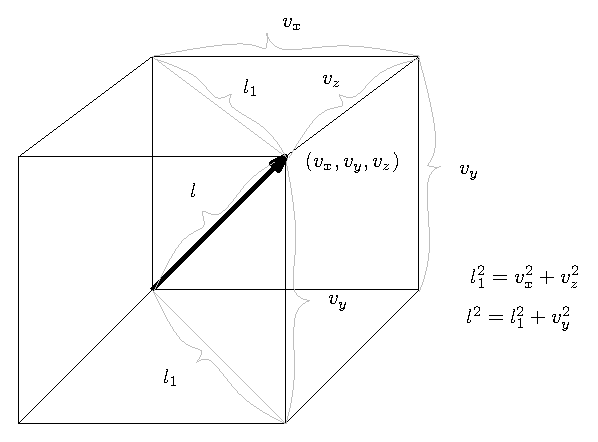
\includegraphics[width=7cm]{Math_vector/3dVectorLength.eps}
\end{figure}

\end{frame}
%%%%%%%%%%%%%%%%%%%%%%%%%%%%%%%%%%%%%%%%%%%%%%%%%%%%%%%%%


%%%%%%%%%%%%%%%%%%%%%%%%%%%%%%%%%%%%%%%%%%%%%%%%%%%%%%%%%
\begin{frame}{벡터의 정규화}
\begin{itemize}
	\item 정규화
	\begin{itemize}
	\item 단위 벡터는 길이가 1인 벡터.
	\item 어떤 벡터의 방향과 일치하는 단위벡터를 구하는 작업은 종종 많은 응용에서 필요.
	\item 이러한 작업은 벡터의 길이를 1로 만드는 것과 같다.
	\item 이를 정규화(normalization)이라고 한다.
	\end{itemize}
\end{itemize}

\begin{figure}
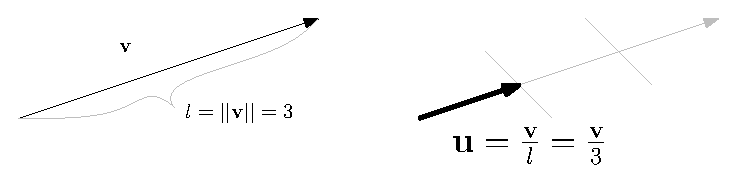
\includegraphics[width=8cm]{Math_vector/unitVector.eps}
\end{figure}
\end{frame}
%%%%%%%%%%%%%%%%%%%%%%%%%%%%%%%%%%%%%%%%%%%%%%%%%%%%%%%%%



\end{document}

